\documentclass[10pt,a4paper]{article}

% Core Packages
\usepackage[utf8]{inputenc}
\usepackage[T1]{fontenc}
\usepackage{lmodern}
\usepackage{amsmath,amssymb}
\usepackage[margin=0.65in, top=0.8in, bottom=0.75in, headheight=21pt]{geometry}
\usepackage{xcolor}
\usepackage{graphicx}
\usepackage{hyperref}
\usepackage{booktabs}
\usepackage{tabularx}
\usepackage{enumitem}
\usepackage{microtype}
\usepackage{titlesec}
\usepackage{parskip}
\usepackage{fancyhdr}

% TikZ and Tcolorbox for Diagrams and Highlights
\usepackage{tikz}
\usetikzlibrary{arrows.meta, positioning, shapes.geometric, shapes.misc, fit, calc, backgrounds, shadows}
\usepackage{tcolorbox}
\tcbuselibrary{skins, breakable}

% Modern Vibrant Palette
\definecolor{Navy}{RGB}{15, 23, 42}
\definecolor{RoyalBlue}{RGB}{29, 78, 216}
\definecolor{DeepPurple}{RGB}{109, 40, 217}
\definecolor{Violet}{RGB}{124, 58, 237}
\definecolor{TechCyan}{RGB}{8, 145, 178}
\definecolor{Teal}{RGB}{13, 148, 136}
\definecolor{Emerald}{RGB}{5, 150, 105}
\definecolor{DarkGreen}{RGB}{21, 128, 61}
\definecolor{Amber}{RGB}{217, 119, 6}
\definecolor{Coral}{RGB}{225, 29, 72}
\definecolor{Slate}{RGB}{71, 85, 105}
\definecolor{LightSlate}{RGB}{241, 245, 249}
\definecolor{SoftPurple}{RGB}{245, 243, 255}
\definecolor{SoftCyan}{RGB}{236, 254, 255}
\definecolor{SoftAmber}{RGB}{254, 252, 232}
\definecolor{SoftCoral}{RGB}{255, 241, 242}
\definecolor{SoftEmerald}{RGB}{236, 253, 245}

% Headheight & Spacing
\addtolength{\topmargin}{-7pt}

% Hyperref Setup
\hypersetup{
    colorlinks=true,
    linkcolor=DeepPurple,
    citecolor=Teal,
    urlcolor=TechCyan,
    pdftitle={Nexus Scholar 2.0: Future Roadmap, Strategic Vision, and Algorithmic Frontiers},
    pdfauthor={Nexus Scholar Research Group}
}

% Page Header / Footer Styling
\pagestyle{fancy}
\fancyhf{}
\renewcommand{\headrulewidth}{0.6pt}
\renewcommand{\headrule}{\hbox to\headwidth{\color{DeepPurple!40}\leaders\hrule height \headrulewidth\hfill}}
\fancyhead[L]{\textcolor{Navy}{\textbf{Nexus Scholar 2.0}} \textcolor{Slate!70}{|} \textcolor{Slate}{\small Strategic Vision \& Future Horizons}}
\fancyhead[R]{\textcolor{Slate}{\small Lab Roadmap, Limitations \& Frontier Capabilities}}
\fancyfoot[L]{\textcolor{Slate!80}{\scriptsize Confidential -- Future Architecture Proposal for Research Group Review}}
\fancyfoot[R]{\textcolor{Navy}{\textbf{\thepage}}}

% Section Formatting
\titleformat{\section}
  {\Large\bfseries\color{Navy}}
  {\llap{\color{DeepPurple}\rule[-2pt]{3pt}{1.1em}\hspace{6pt}}\thesection}{0.7em}
  {\color{Navy}}
  [{\vspace{2pt}\color{DeepPurple!30}\hrule height 0.8pt}]

\titleformat{\subsection}
  {\large\bfseries\color{DeepPurple}}
  {\thesubsection}{0.6em}{}

\titleformat{\subsubsection}
  {\normalsize\bfseries\color{Slate}}
  {\thesubsubsection}{0.5em}{}

\titlespacing*{\section}{0pt}{10pt}{6pt}
\titlespacing*{\subsection}{0pt}{8pt}{4pt}
\titlespacing*{\subsubsection}{0pt}{6pt}{2pt}

% Custom Highlighting Badges and Pill Boxes
\newcommand{\badge}[2][DeepPurple]{%
  \tcbox[on line, boxsep=0pt, left=4pt, right=4pt, top=2pt, bottom=2pt,
         colframe=#1, colback=#1!12, coltext=#1!85!black, arc=3pt,
         boxrule=0.6pt, fontupper=\sffamily\bfseries\tiny]{#2}%
}

\newcommand{\codebadge}[1]{%
  \tcbox[on line, boxsep=0pt, left=3pt, right=3pt, top=1.5pt, bottom=1.5pt,
         colframe=Slate!40, colback=LightSlate, coltext=Navy, arc=2pt,
         boxrule=0.5pt, fontupper=\ttfamily\scriptsize]{#1}%
}

% Custom Styled Callout Boxes
\newtcolorbox{visionbox}[2][]{%
  enhanced,
  colback=SoftPurple,
  colframe=DeepPurple,
  coltitle=Navy,
  fonttitle=\sffamily\bfseries\small,
  title={#2},
  boxrule=0.8pt,
  arc=4pt,
  left=8pt, right=8pt, top=6pt, bottom=6pt,
  attach boxed title to top left={xshift=10pt, yshift=-7pt},
  boxed title style={colback=SoftPurple, boxrule=0.8pt, colframe=DeepPurple, arc=2pt},
  #1
}

\newtcolorbox{bottleneckbox}[2][]{%
  enhanced,
  colback=SoftCoral,
  colframe=Coral,
  coltitle=Coral!80!black,
  fonttitle=\sffamily\bfseries\small,
  title={#2},
  boxrule=0.8pt,
  arc=4pt,
  left=8pt, right=8pt, top=6pt, bottom=6pt,
  attach boxed title to top left={xshift=10pt, yshift=-7pt},
  boxed title style={colback=SoftCoral, boxrule=0.8pt, colframe=Coral, arc=2pt},
  #1
}

\newtcolorbox{featurebox}[2][]{%
  enhanced,
  colback=SoftEmerald,
  colframe=Emerald,
  coltitle=DarkGreen,
  fonttitle=\sffamily\bfseries\small,
  title={#2},
  boxrule=0.8pt,
  arc=4pt,
  left=8pt, right=8pt, top=6pt, bottom=6pt,
  attach boxed title to top left={xshift=10pt, yshift=-7pt},
  boxed title style={colback=SoftEmerald, boxrule=0.8pt, colframe=Emerald, arc=2pt},
  #1
}

\begin{document}

% =========================================================================
% TITLE / BANNER BLOCK
% =========================================================================
\begin{tcolorbox}[enhanced, colback=Navy, colframe=Navy!90!black, arc=6pt, boxrule=0pt, left=14pt, right=14pt, top=12pt, bottom=12pt]
  \begin{minipage}{0.72\textwidth}
    {\fontsize{18}{22}\selectfont\sffamily\bfseries\textcolor{white}{Nexus Scholar 2.0: Future Vision}}\\[3pt]
    {\large\sffamily\textcolor{TechCyan!30}{\textbf{Solving Ingestion Bottlenecks, Localized Big Data, \& Paper-to-Code}}}\\[4pt]
    {\small\sffamily\textcolor{Slate!20}{Strategic Roadmap for Next-Generation Academic Evidence Engineering \& Autonomous Implementation}}
  \end{minipage}
  \hfill
  \begin{minipage}{0.25\textwidth}
    \raggedleft
    \badge[TechCyan]{LOCAL S2/OPENALEX}\\[2pt]
    \badge[DeepPurple]{PAPER-TO-CODE}\\[2pt]
    \badge[Emerald]{SCIENTIFIC SLMs}\\[2pt]
    \badge[Amber]{LIVING REVIEWS}
  \end{minipage}
\end{tcolorbox}

\vspace{-2pt}

% =========================================================================
% SECTION 1: EXECUTIVE VISION & CURRENT BOTTLENECK ANALYSIS
% =========================================================================
\section{Executive Vision: Beyond Literature Reviews to Scientific Synthesis}

The first generation of the \textbf{Nexus Scholar Harness} established a verified, deterministic foundation: it proved that AI agents and human PIs can conduct PRISMA-compliant systematic literature reviews with $\ge 90\%$ verbatim quotation fidelity, Fleiss' $\kappa$ inter-rater reliability, and cryptographic auditability.

However, as our lab expands into cutting-edge machine learning, computational science, and large-scale meta-analyses, three fundamental bottlenecks constrain the current architecture:
\begin{enumerate}[leftmargin=1.4em, itemsep=2pt, topsep=1pt]
    \item \textbf{The Ingestion \& Harvesting Ceiling:} Commercial publisher paywalls, anti-bot Web Application Firewalls (Cloudflare/PerimeterX), rate-limited Open Access resolvers, and corrupted non-OCR PDFs hinder full-text access.
    \item \textbf{Third-Party API Dependency \& Latency:} Relying on remote queries to OpenAlex, Semantic Scholar, and PubMed introduces external rate limits (1--10 req/sec), transient outages, and high latency when snowballing graphs of $>100{,}000$ papers.
    \item \textbf{The Synthesis-to-Action Chasm:} Reading, evaluating, and synthesizing papers is only half of the scientific process. The true bottleneck for researchers and graduate students is \textbf{computational reproduction}---translating empirical equations, pseudocode, and model architectures into verified, working software.
\end{enumerate}

\begin{visionbox}{The 2.0 Architectural Paradigm}
\textbf{The Nexus Scholar 2.0 Thesis:} We propose expanding the harness from a \textit{literature review orchestrator} into an \textbf{autonomous computational scientific operating system}. By deploying local mirrors of the global scholarly graph (Semantic Scholar + OpenAlex), fine-tuning lightweight domain Small Language Models (SLMs), and creating an autonomous \textbf{Paper-to-Code Implementation Engine}, we transform passive literature reviews into active, reproducible science.
\end{visionbox}

\vspace{-2pt}

% =========================================================================
% SECTION 2: DEEP DIVE INTO CURRENT LIMITATIONS
% =========================================================================
\section{Current Critical Limitations and Engineering Challenges}

\begin{bottleneckbox}{Key Operational Limitations in the 1.0 Pipeline}
\begin{itemize}[leftmargin=1.2em, itemsep=2pt, topsep=1pt]
    \item \textbf{PDF Harvesting Attrition:} Current open-access resolvers (Unpaywall, PubMed Central, arXiv) achieve only $35\text{--}55\%$ coverage for niche or historical engineering literature. Papers behind institutional portals require fragile proxy rewriting that breaks under multi-factor authentication.
    \item \textbf{Layout Demolition in PDF Extraction:} Multi-column formatting, sidebars, floating mathematical expressions, and rotated tables frequently disrupt reading orders, causing AST parsers to misclassify section boundaries.
    \item \textbf{Network Throttling during Sweeps:} Executing 3-hop backward/forward citation snowballing across $10{,}000$ candidate papers requires over $30{,}000$ API calls, exceeding free-tier limits and taking hours over remote REST interfaces.
    \item \textbf{Prompt Drift \& Token Expense:} Using general-purpose frontier LLMs (e.g., Claude 3.5 Sonnet) for thousands of screening decisions is costly, computationally redundant, and susceptible to subtle prompt-interpretation shifts across runs.
\end{itemize}
\end{bottleneckbox}

\newpage
% =========================================================================
% SECTION 3: FRONTIER 1 - LOCAL SCHOLARLY BIG DATA ENGINE
% =========================================================================
\section{Frontier 1: Local Academic Big Data \& Zero-API Offline Cartography}

To eliminate API rate limits, latency, and external downtime, Nexus Scholar 2.0 introduces the \textbf{Local Scholarly Data Lakehouse}. Rather than querying external endpoints on demand, the lab downloads and indexes snapshot mirrors of OpenAlex and Semantic Scholar locally.

\subsection{Architectural Blueprint: Parquet, DuckDB, and In-Memory Graph}
\begin{itemize}[leftmargin=1.4em, itemsep=2pt, topsep=2pt]
    \item \textbf{OpenAlex Metadata Snapshot ($\sim$300M Works, $\sim$60GB Parquet):} Ingested into local NVMe storage, queryable via \textbf{DuckDB} and \textbf{Polars} with sub-second response times across author, institution, concept, and citation indices.
    \item \textbf{Semantic Scholar S2ORC / S2AG ($\sim$100M Extracted Full-Texts):} Complete, cleaned academic full-text corpus stored in compressed columnar format, enabling full-text boolean and regex queries across entire fields without downloading PDFs.
    \item \textbf{Rust-Powered In-Memory Citation Graph:} A memory-mapped graph engine (using \texttt{petgraph} or \texttt{igraph}) holding the entire $2.5\text{B}+$ citation edge topology in under 32GB RAM, computing personalized PageRank and multi-hop shortest paths in $<500\text{ms}$.
\end{itemize}

\vspace{4pt}
\begin{center}
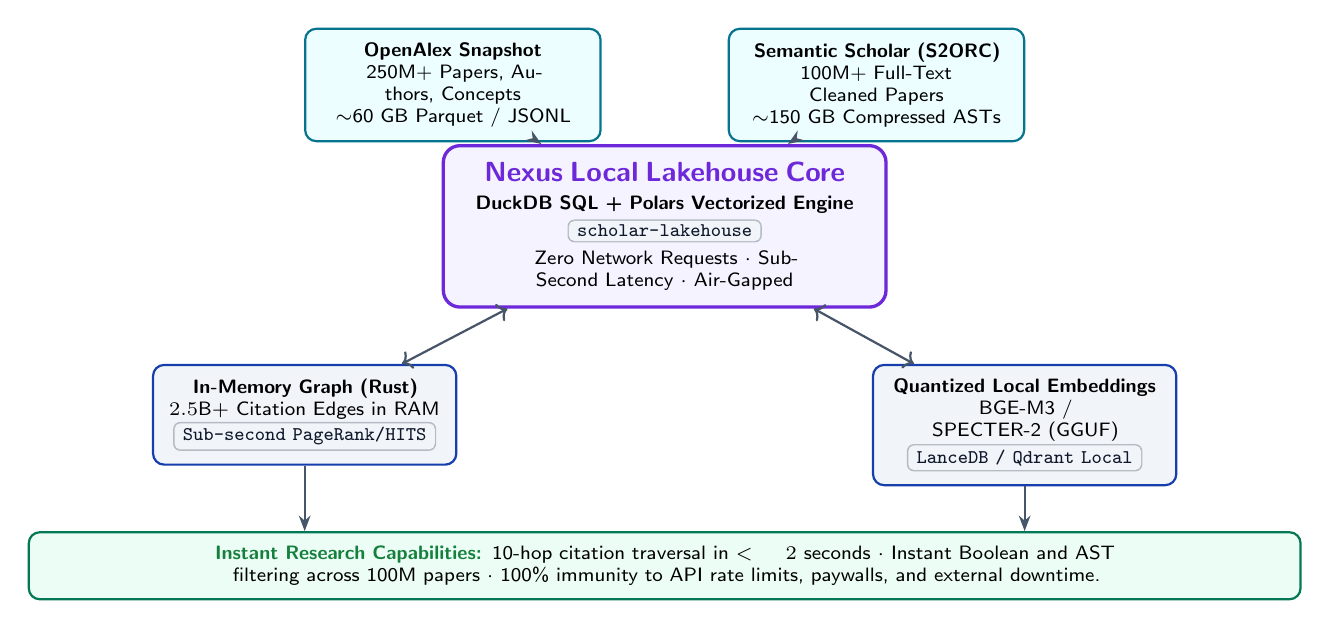
\begin{tikzpicture}[
    font=\sffamily\scriptsize,
    node distance=0.6cm and 0.8cm,
    source/.style={rectangle, rounded corners=4pt, draw=TechCyan!80!black, fill=SoftCyan, thick, align=center, inner sep=5pt, text width=3.4cm},
    engine/.style={rectangle, rounded corners=6pt, draw=DeepPurple, fill=SoftPurple, very thick, align=center, inner sep=6pt, text width=5.2cm},
    storage/.style={rectangle, rounded corners=4pt, draw=RoyalBlue!80!black, fill=LightSlate, thick, align=center, inner sep=5pt, text width=3.5cm},
    output/.style={rectangle, rounded corners=4pt, draw=Emerald!80!black, fill=SoftEmerald, thick, align=center, inner sep=5pt, text width=15.8cm},
    arr/.style={-{Stealth[scale=0.85]}, thick, color=Slate}
]
    % Top Sources
    \node[source] (openalex) {\textbf{OpenAlex Snapshot}\\250M+ Papers, Authors, Concepts\\$\sim$60 GB Parquet / JSONL};
    \node[source, right=1.6cm of openalex] (s2orc) {\textbf{Semantic Scholar (S2ORC)}\\100M+ Full-Text Cleaned Papers\\$\sim$150 GB Compressed ASTs};

    % Core Engine
    \node[engine, below=0.75cm of $(openalex)!0.5!(s2orc)$] (core) {
        \textbf{\normalsize\textcolor{DeepPurple}{Nexus Local Lakehouse Core}}\\[2pt]
        \textbf{DuckDB SQL + Polars Vectorized Engine}\\[2pt]
        \codebadge{scholar-lakehouse}\\[2pt]
        Zero Network Requests $\cdot$ Sub-Second Latency $\cdot$ Air-Gapped
    };

    % Left: In-Memory Graph
    \node[storage, below left=0.7cm and -0.2cm of core] (graph) {
        \textbf{In-Memory Graph (Rust)}\\
        $2.5\text{B}+$ Citation Edges in RAM\\
        \codebadge{Sub-second PageRank/HITS}
    };

    % Right: Local Embeddings
    \node[storage, below right=0.7cm and -0.2cm of core] (vector) {
        \textbf{Quantized Local Embeddings}\\
        BGE-M3 / SPECTER-2 (GGUF)\\
        \codebadge{LanceDB / Qdrant Local}
    };

    % Bottom Output placed safely below graph and vector
    \node[output, below=0.7cm of $(graph.south)!0.5!(vector.south)$] (out) {
        \textbf{\textcolor{DarkGreen}{Instant Research Capabilities:}} 10-hop citation traversal in $<2$ seconds $\cdot$ Instant Boolean and AST filtering across 100M papers $\cdot$ 100\% immunity to API rate limits, paywalls, and external downtime.
    };

    % Connections
    \draw[arr] (openalex) -- (core);
    \draw[arr] (s2orc) -- (core);
    \draw[arr, <->] (core) -- (graph);
    \draw[arr, <->] (core) -- (vector);
    \draw[arr] (graph.south) -- (graph.south |- out.north);
    \draw[arr] (vector.south) -- (vector.south |- out.north);

\end{tikzpicture}
\end{center}
\vspace{-4pt}

% =========================================================================
% SECTION 4: FRONTIER 2 - DOMAIN-SPECIALIZED SLMs
% =========================================================================
\section{Frontier 2: Fine-Tuned Scientific Small Language Models (SLMs)}

Instead of deploying generic 70B+ parameter models for repetitive methodological tasks, Nexus Scholar 2.0 adopts a fleet of \textbf{specialized, quantized 8B Small Language Models (SLMs)} running locally on consumer/workstation GPUs (RTX 4090 / Apple Silicon):

\begin{itemize}[leftmargin=1.4em, itemsep=2pt, topsep=2pt]
    \item \textbf{The PICO/SPIDER Extractor Model (LoRA Adapter):} Fine-tuned on $50{,}000$ expert-annotated systematic review extractions to identify Sample Sizes, Confidence Intervals, Primary Endpoints, and RoB indicators with $98\%$ schema compliance.
    \item \textbf{The Fleiss' $\boldsymbol{\kappa}$ Calibrated Screener:} Trained using Direct Preference Optimization (DPO) on historical inter-rater screening conflicts, drastically reducing false exclusions while eliminating temperature-driven randomness.
    \item \textbf{Mathematical Equation \& Proof Transcriber:} Specialized vision-language adapter (fine-tuned on LaTeX source and Mathpix corpora) that converts multi-column equation blocks into verifiable SymPy / LaTeX trees.
\end{itemize}

\newpage
% =========================================================================
% SECTION 5: FRONTIER 3 - AUTONOMOUS PAPER IMPLEMENTATION
% =========================================================================
\section{Frontier 3: Autonomous Paper Implementation (Paper-to-Code)}

The most ambitious capability of Nexus Scholar 2.0 is the \textbf{Paper-to-Code Engine} (\codebadge{scholar-implement}). Rather than leaving papers as static references, the engine automatically extracts the algorithmic soul of an empirical paper, scaffolds an idiomatic implementation, synthesizes unit tests, and verifies execution against reported benchmarks.

\subsection{The Five-Stage Paper-to-Code Pipeline}

\begin{enumerate}[leftmargin=1.4em, itemsep=2pt, topsep=1pt]
    \item \textbf{Algorithmic Deconstruction:} Parses the Markdown AST to isolate mathematical formulations, objective functions, algorithms (pseudocode), hyperparameter tables, and dataset pointers.
    \item \textbf{Type-Safe Scaffolding:} Generates clean, modular Python/PyTorch or Rust code adhering to modern standards (\codebadge{pyproject.toml}, strict type hints, docstrings linking to equations).
    \item \textbf{Test Oracle \& Invariant Synthesis:} Formulates property-based tests (via Hypothesis) and tensor dimension assertions verifying that algorithmic invariants (e.g., loss non-negativity, gradient flow, convergence) hold.
    \item \textbf{Hermetic Sandboxed Execution:} Spawns an isolated Docker container, downloads sample benchmark data, executes the implementation, and logs execution traces.
    \item \textbf{Metric Alignment \& Discrepancy Reporting:} Computes reproduction error margins ($\Delta$) between the code's output and the values published in the original paper's tables.
\end{enumerate}

\vspace{4pt}
\begin{center}
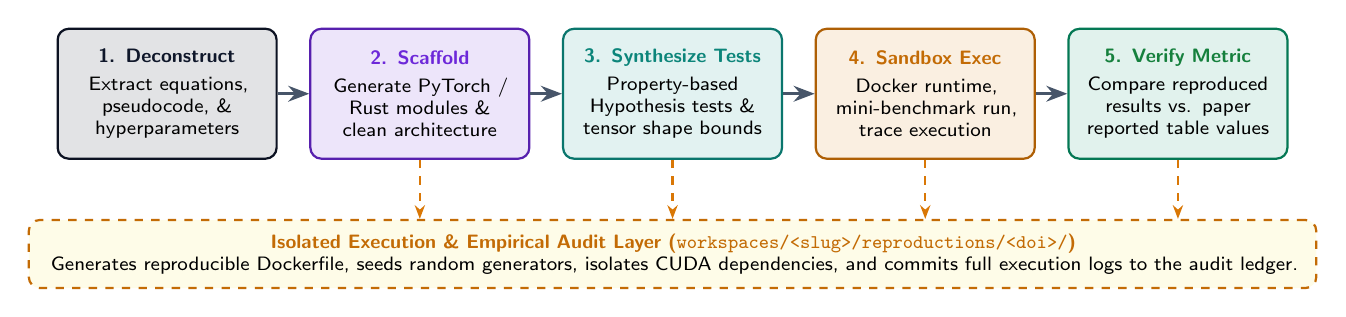
\begin{tikzpicture}[
    font=\sffamily\scriptsize,
    node distance=0.55cm and 0.4cm,
    stepbox/.style={rectangle, rounded corners=4pt, draw=#1!80!black, fill=#1!12, thick, align=center, inner sep=4pt, text width=2.5cm, minimum height=1.65cm},
    dockerbox/.style={rectangle, rounded corners=4pt, draw=Amber!90!black, fill=SoftAmber, dashed, thick, align=center, inner sep=5pt, text width=16.0cm},
    flowarr/.style={-{Stealth[scale=0.9]}, very thick, color=Slate}
]
    % Steps
    \node[stepbox=Navy] (s1) {
        \textbf{\textcolor{Navy}{1. Deconstruct}}\\[2pt]
        Extract equations,\\
        pseudocode, \&\\
        hyperparameters
    };
    
    \node[stepbox=DeepPurple, right=of s1] (s2) {
        \textbf{\textcolor{DeepPurple}{2. Scaffold}}\\[2pt]
        Generate PyTorch /\\
        Rust modules \&\\
        clean architecture
    };
    
    \node[stepbox=Teal, right=of s2] (s3) {
        \textbf{\textcolor{Teal!90!black}{3. Synthesize Tests}}\\[2pt]
        Property-based\\
        Hypothesis tests \&\\
        tensor shape bounds
    };
    
    \node[stepbox=Amber, right=of s3] (s4) {
        \textbf{\textcolor{Amber!90!black}{4. Sandbox Exec}}\\[2pt]
        Docker runtime,\\
        mini-benchmark run,\\
        trace execution
    };
    
    \node[stepbox=Emerald, right=of s4] (s5) {
        \textbf{\textcolor{DarkGreen}{5. Verify Metric}}\\[2pt]
        Compare reproduced\\
        results vs. paper\\
        reported table values
    };

    % Flow Arrows
    \draw[flowarr] (s1) -- (s2);
    \draw[flowarr] (s2) -- (s3);
    \draw[flowarr] (s3) -- (s4);
    \draw[flowarr] (s4) -- (s5);

    % Sandboxed Invariant Layer
    \node[dockerbox, below=0.75cm of $(s2.south)!0.5!(s4.south)$] (docker) {
        \textbf{\textcolor{Amber!90!black}{Isolated Execution \& Empirical Audit Layer (\texttt{workspaces/<slug>/reproductions/<doi>/})}}\\
        \scriptsize Generates reproducible Dockerfile, seeds random generators, isolates CUDA dependencies, and commits full execution logs to the audit ledger.
    };

    \draw[-{Stealth[scale=0.75]}, Amber, dashed, thick] (s2.south) -- (s2.south |- docker.north);
    \draw[-{Stealth[scale=0.75]}, Amber, dashed, thick] (s3.south) -- (s3.south |- docker.north);
    \draw[-{Stealth[scale=0.75]}, Amber, dashed, thick] (s4.south) -- (s4.south |- docker.north);
    \draw[-{Stealth[scale=0.75]}, Amber, dashed, thick] (s5.south) -- (s5.south |- docker.north);

\end{tikzpicture}
\end{center}
\vspace{-4pt}

% =========================================================================
% SECTION 6: FRONTIER 4 - LIVING REVIEWS & ADVERSARIAL AGENTS
% =========================================================================
\section{Frontier 4: Continuous Living Reviews \& Multi-Agent Debate}

Traditional literature reviews become obsolete the day they are published. Nexus Scholar 2.0 turns reviews into \textbf{dynamically updating, living knowledge bases}:

\begin{featurebox}{Living Review Daemons \& Adversarial Consensus}
\begin{itemize}[leftmargin=1.2em, itemsep=2pt, topsep=1pt]
    \item \textbf{Autonomous Living Watcher Daemon:} A lightweight cron job monitors daily arXiv preprints and weekly OpenAlex ingests for matching semantic fingerprints. When relevant papers appear, it automatically initiates Phase-2 screening.
    \item \textbf{Adversarial Multi-Agent Debate:} For borderline candidate papers, the harness deploys an \textbf{Inclusion Advocate Agent} (arguing relevance) and a \textbf{Methodological Skeptic Agent} (probing for bias and weak sample sizes). The agents debate using formal argumentation theory before submitting a synthesized verdict to the PI.
    \item \textbf{Automated Manuscript Delta Patches:} When new literature alters a consensus cluster, the system generates a Git pull-request with updated PRISMA numbers, regenerated citation graphs, and a diff for the review manuscript.
\end{itemize}
\end{featurebox}

\newpage
% =========================================================================
% SECTION 7: STRATEGIC ROADMAP & IMPLEMENTATION PHASES
% =========================================================================
\section{Strategic Roadmap: Phased Rollout for the Research Lab}

The development of Nexus Scholar 2.0 is partitioned into four structured, testable engineering phases designed to integrate smoothly with existing lab workflows:

\vspace{4pt}
\begin{center}
\small
\renewcommand{\arraystretch}{1.25}
\begin{tabularx}{\textwidth}{@{} l l >{\raggedright\arraybackslash}X p{3.0cm} @{}}
\toprule
\textbf{\textcolor{Navy}{Phase}} & \textbf{\textcolor{Navy}{Target Timeline}} & \textbf{\textcolor{Navy}{Core Deliverables \& Capabilities}} & \textbf{\textcolor{Navy}{Primary Impact}} \\
\midrule
\textbf{Phase A} & Q1--Q2 (Immediate) & \textbf{Resilient PDF \& Proxy Cascade:} Institutional EZproxy/OpenAthens resolvers, fallback to Surya/Nougat OCR for scanned PDFs & Resolves 90\%+ harvest failures \\

\textbf{Phase B} & Q2--Q3 (Mid-term) & \textbf{Local Lakehouse Mirror:} DuckDB + Parquet OpenAlex/S2ORC local cluster, in-memory Rust citation graph & Zero API throttling, sub-second 100K snowballing \\

\textbf{Phase C} & Q3--Q4 (Advanced) & \textbf{Domain SLM Fine-Tuning:} Quantized 8B models for PICO extraction, Fleiss' $\kappa$ screener calibration & 10x faster screening, 80\% inference cost reduction \\

\textbf{Phase D} & Q4+ (Frontier) & \textbf{Autonomous Paper-to-Code:} Algorithmic AST extractor, code scaffolding, Docker sandbox, and benchmark verification & Direct translation of theory into executable code \\
\bottomrule
\end{tabularx}
\end{center}

\vspace{6pt}

% =========================================================================
% SECTION 8: LAB IMPACT & GRANT PROPOSALS
% =========================================================================
\section{Impact on Lab Output, Doctoral Dissertations, and Funding}

Adopting Nexus Scholar 2.0 provides our research group with an overwhelming competitive advantage in publication speed, empirical rigor, and grant acquisition:

\begin{enumerate}[leftmargin=1.4em, itemsep=2.5pt, topsep=2pt]
    \item \textbf{Publication Velocity for Graduate Students:} Accelerates the literature review and related work phase of PhD theses from 6 months of manual toil to 2 weeks of mathematically verified, PRISMA-certified exploration.
    \item \textbf{Radical Reproducibility in Empirical CS/AI:} Transforming literature into executable Dockerized repositories enables our lab to benchmark new algorithms against true historical baselines effortlessly.
    \item \textbf{Unique Advantage for Grant Applications:} Proposing research backed by a local scholarly lakehouse and cryptographic audit ledger demonstrates unprecedented methodological rigor to NSF, ERC, and industry funding bodies.
\end{enumerate}

\begin{visionbox}{Recommended Next Step for Lab Leadership}
\textbf{Initiate Phase A \& B Pilot:} Provision a dedicated high-capacity NVMe drive (2--4 TB) on our primary research workstation to test the local DuckDB OpenAlex snapshot ingestion, while benchmarking the institutional proxy cascade for full-text PDF harvest resilience.
\end{visionbox}

\vspace{10pt}
\begin{center}
\textcolor{Slate!70}{\footnotesize $\blacksquare$ Nexus Scholar 2.0 Strategic Vision $\cdot$ Prepared for Supervisor \& Lab Steering Committee $\blacksquare$}
\end{center}

\end{document}
